section{Equations}


The SMODERP2D episodic rainfall-runoff/erosion model was used for the
investigation presented here. The 2D model is based on a 1D profile version, in
which the surface runoff and the erosion were typically calculated in several
1D profiles representing the main flow path in the hillslope \cite{Dostal2000}.
The current generation of the SMODERP2D model is pixel distributed, and is
implemented in python in order to be compatible with most GIS software. The
development is presented on the github platform at
\href{https://github.com/storm-fsv-cvut/smoderp2d}{github.com/storm-fsv-cvut/smoderp2d}.

The SMODERP2D model is primarily designed for surface runoff and erosion
computation. The surface flow routing in the model is based on the digital
elevation model (DEM). DEM also controls the spatial discretization of the
model. The principle of the model is the cell-by-cell mass balance calculated
in each time step. The change in the water level of the shear flow in any cell
in time is controlled using the equation: 
\begin{equation} 
\frac{\mathrm{d}h}{\mathrm{d}t} = es_{i,t-1} + q^{in}_{i,t-1} - inf_{i,t-1} - q^{out}_{i,t-1},
\label{eq:bilance}
\end{equation}
where h is the surface water level (L), qin and qout are the sheet overland
inflow and outflow into and out of a given raster cell ($\mathrm{L.t^{-1}}$),
ep is the effective precipitation intensity (the potential precipitation
reduced by the interception zone and the surface retention)
($\mathrm{L.t^{-1}}$), and inf is the infiltration rate ($\mathrm{L.t^{-1}}$).
The kinematic wave approach is used in the calculation of the overland flow.
The momentum is therefore expressed by the power-law:

\begin{equation} 
q = ah^b
\label{eq:powerlaw}
\end{equation}
where a and b are power-law parameters. Equation \ref{eq:powerlaw} can be expressed in the form of the Manning–Strickler formula


\begin{equation} 
q = n^{-1} s^Y h^b,
\label{eq:powerlaw}
\end{equation}
where n is roughness,  Y  empirical parameter and s is the surface slope ($\mathrm{L.L^{-1}}$).

The infiltration component of Equation \ref{eq:bilance} is calculated by the
Philip infiltration equation \citep{philip1957}
\begin{equation} 
inf = \frac{1}{2}St^{-1/2}+K_s.
\label{eq:infiltration}
\end{equation} 

where S stands for sorptivity ($\mathrm{L.t^{1/2}}$) and ($\mathrm{K_s}$)
stands for saturation hydraulic conductivity ($\mathrm{L.t^{-1}}$).

The SMODERP2D model is subjected to uniform rainfall. The potential
precipitation is reduced due to surface retention. The surface retention is the
storage that needs to be filled before surface runoff can occur. 

The flow routing of the surface runoff is based on the D8 one-direction flow
algorithm \cite{o1984extraction}. The inflow to cell i is defined as the sum of the sheet
outflows from the adjacent cells, as:

\begin{equation} 
q^{in}_{i,t-1} = \sum_j^m q^{out}_{j,t-1}, 
\label{eq:d8}
\end{equation} 
where j is the index of the adjacent up-slope cells identified by the D8 flow
algorithm.

The time derivative in Equation \ref{eq:bilance} is calculated using an
explicit method. The computation is therefore sensitive to the size of the time
step. The size of the time step is controlled by the Courant criterion, which
needs to be kept below the theoretical maximum value of 1, while the maximum
value in practise is lower than 1 
\cite{zhang1989modeling, esteves2000overland}.


The sheet flow water level of the next time t + 1 step in Equation
\ref{eq:bilance} which incorporates the sum \ref{eq:d8} is calculated with the
explicit time discretisation scheme for cell i as:
\begin{equation} 
h_{i,t} =h_{i,t} + \mathrm{d}t (es_{i,t-1} + \sum_j^m q^{out}_{j,t-1}-
inf_{i,t-1} - q^{out}_{i,t-1}),
\label{eq:bilance}
\end{equation}

\section{Rill Flow}

The rill flow is also included in the calculation. In SMODERP2D, rill flow in a
cell occurs if $h>h_{crit}$, where $h_{crit}$ is the critical water level. The
water flow corresponding to the water level above the critical water level has
enough energy to start to carry the soil particles and to create a rill.

The critical water level $h_{crit}$ is calculated as:
\begin{equation}
  h_{crit} = MIN(h_{v_{crit}},h_{\tau_{crit}}),
  \label{eq:critdef}
\end{equation}
where $h_{v_{crit}}$ is the water corresponding to the critical velocity, and
$h_{\tau_{crit}}$ is the water level corresponding to the critical shear
stress.  As shown in Formula \ref{eq:critdef}, $h_{crit}$ uses several values
obtained with a different approach. This approach is adopted in order to remain
on the safe side of the emergence of a rill, since $h_{v_{crit}}$ is more
sensitive to the sheet flow velocity and $h_{\tau_{crit}}$ is more sensitive to
the slope of the soil surface. 

When the condition $h>h_{crit}$ is fulfilled, a rill starts to develop in a
given cell and $h_{sheet}=h_{crit}$. In SMODERP2D, the rill is a dynamic component and
can increase as the rill flow increases. The rill volume is controlled by the
volume of water corresponding to the rill water level $h_{rill}$. This volume is
calculated as:


\begin{equation}
  V_{rill} = h_{rill}P,
  \label{eq:rillvol}
\end{equation}

The critical water level $h_{crit}$ is calculated as:
\begin{equation}
  h_{rill} = MAX(h-h_{crit},0),
  \label{eq:hrill}
\end{equation}
P stands for the size of the raster cell. The rill is simplified as a small
channel at the soil surface with a rectangular cross section. The rectangle has
width $b_{rill}$ and rill height $y_{rill} = 0.7b_{rill}$. The rill flow is as
calculated with the Manning equation: 

\begin{equation}
    q_{rill} = \frac{A}{n_{rill}} s^{1/2} R_{rill}^{2/3},
  \label{eq:rillflow}
\end{equation}
where A is the cross section of the rill,  $n_{rill}$ is the roughness in the
rill, s is the surface slope, and  $R_{rill}$  is the hydraulic radius of the
rill. 

As stated above, the size of the rill changes as $h_{rill}$ increases. The
scheme of this change is shown in Figure \ref{fig:rill_plneni}. The change in
the rill flow varies with the change in $R_{rill}$ in Equation
\ref{eq:rillflow}, since $h_{rill}$ increases, and therefore $y_{rill}$ and
$b_{rill}$ also increase. The $R_{rill}$ for an increasing rill is calculated
as:
\begin{equation}
    R_{rill} = \frac{h_{rill}b_{rill}}{2h_{rill}+b_{rill}}  =
    \frac{y_{rill}b_{rill}}{2y_{rill}+b_{rill}},
  \label{eq:rrill}
\end{equation}
where:
\begin{equation}
  b_{rill} = h_{rill}/0.7
  \label{eq:brill}
\end{equation}


\begin{figure}[b]
    \centering
    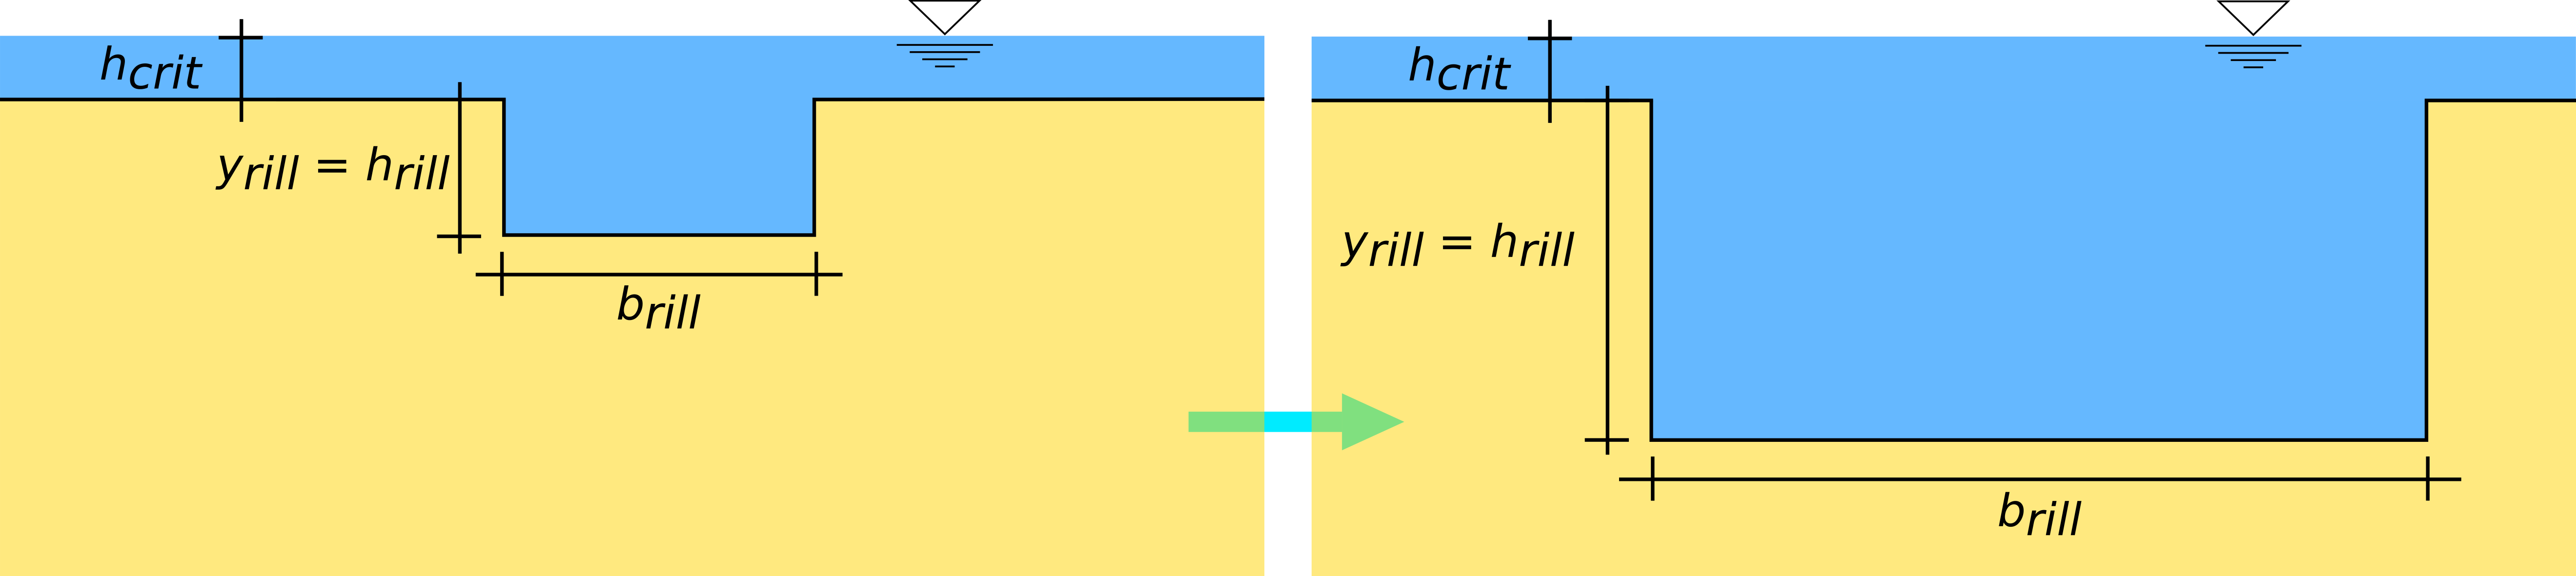
\includegraphics[width=1\linewidth]{./img/rill_schema_plneni.png}
    \caption{Scheme of the rill size during increasing surface runoff.}
    \label{fig:rill_plneni}
\end{figure}


During the recession limb of the hydrograph, the rill size “locks”, and
$h_{rill}$ decreases until the rill is empty. The scheme of the emptying rill
and the rill flow is shown in Figure~\ref{fig:rill_prazdneni}. In this case,
$R_{rill}$ is calculated from fixed $b_{rill}$ and decreasing $h_{rill}$.
$R_{rill}$ for decreasing rill flow is calculated as:
\begin{equation}
    R_{rill} = \frac{h_{rill}b_{rill}}{2h_{rill}+b_{rill}},
  \label{eq:rrill2}
\end{equation}
where:
\begin{equation}
  b_{rill} = y_{rill}/0.7
  \label{eq:brill2}
\end{equation}

\begin{figure}[t]
    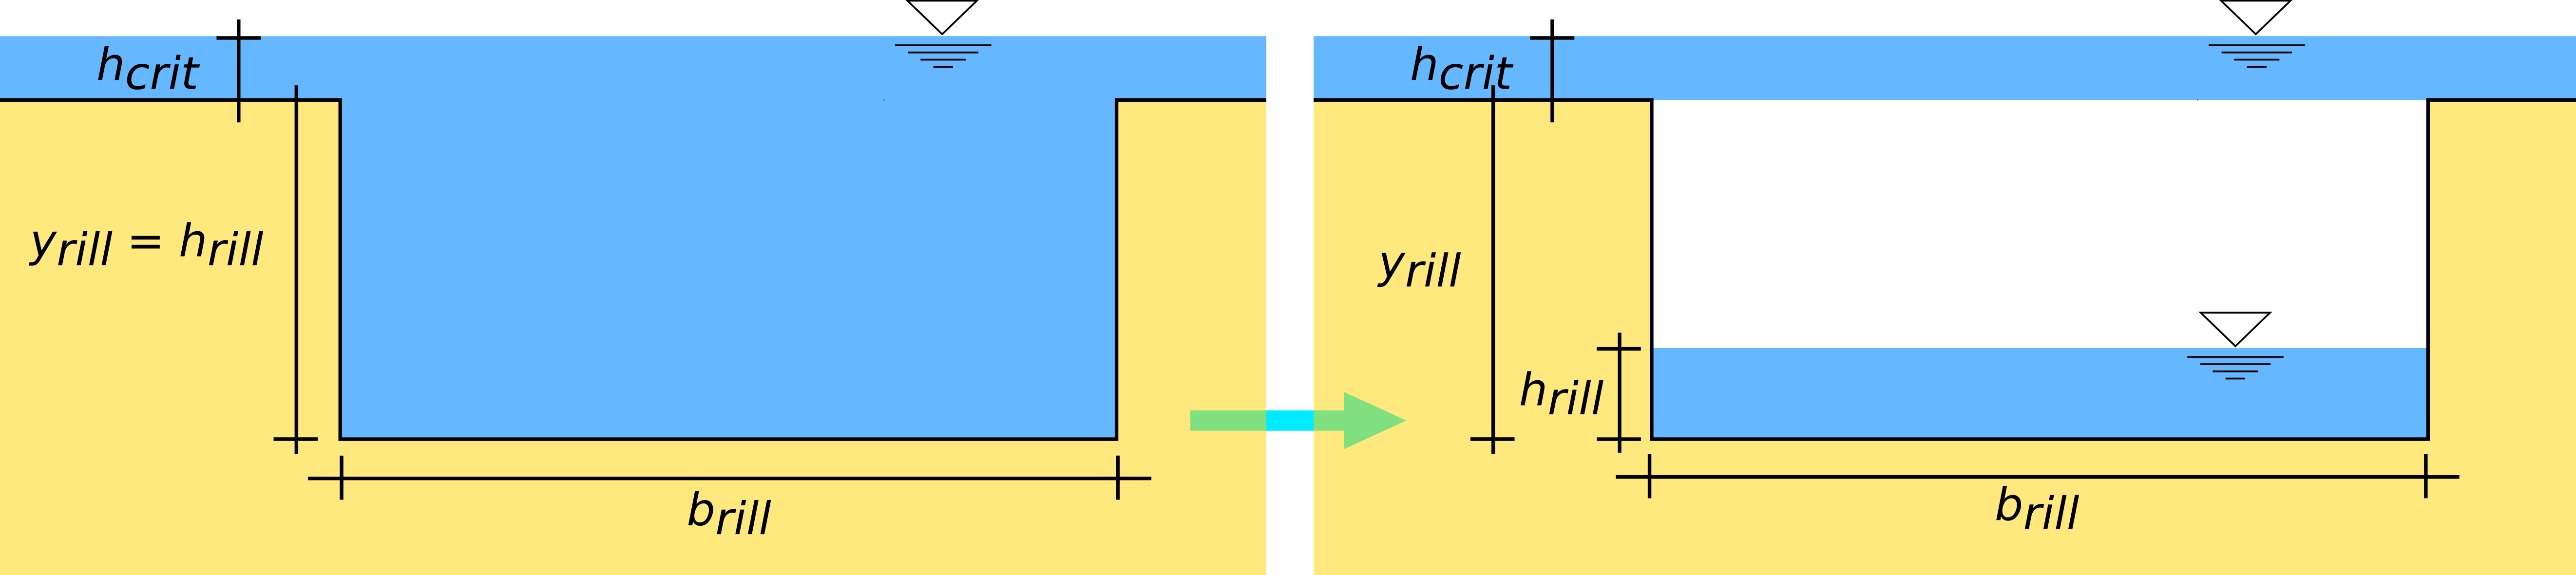
\includegraphics[width=1\linewidth]{./img/rill_schema_prazdneni.png}
    \caption{Scheme of the rill size during the recession limb of the hydrograph.}
    \label{fig:rill_prazdneni}
\end{figure}

The total water balance in cell i, where a rill is developed, is calculated as:

\begin{equation}
    \frac{\mathrm{d}h_i}{\mathrm{d}t} = es_i + q^{in}_{sheet,i}(h_{sheet,i})
    +q^{in}_{rill,i}(h_{rill,i}) - (inf_i + q^{out}_{sheet,i}(h_{sheet,i}) +
    q^{out}_{rill,i}(h_{rill,i}))
    %
    %
    %h_{i,t} =h_{i,t} + \mathrm{d}t (es_{i,t-1} + \sum_j^m q^{out}_{j,t-1}-
    %inf_{i,t-1} - q^{out}_{i,t-1}),
\end{equation}
where:
\begin{equation}
    q^{in}_{sheet,i} = \sum_j^m q^{out}_{sheet, j}(h_{sheet,j}),\quad \mathrm{and}
\end{equation}
\begin{equation}
    q^{in}_{rill,i} = \sum_j^m q^{out}_{rill, j}(h_{rill,j})
\end{equation}

and:
\begin{equation}
   h = h_{rill} + h_{sheet}  
\end{equation}

The rill water level is recalculated to cover the whole cell and not just the
bottom of the rill, as shown in Figures \ref{fig:rill_plneni} and
\ref{fig:rill_prazdneni}.

%
%

%
